% Options for packages loaded elsewhere
\PassOptionsToPackage{unicode}{hyperref}
\PassOptionsToPackage{hyphens}{url}
\PassOptionsToPackage{dvipsnames,svgnames,x11names}{xcolor}
%
\documentclass[
  letterpaper,
  DIV=11,
  numbers=noendperiod]{scrartcl}

\usepackage{amsmath,amssymb}
\usepackage{iftex}
\ifPDFTeX
  \usepackage[T1]{fontenc}
  \usepackage[utf8]{inputenc}
  \usepackage{textcomp} % provide euro and other symbols
\else % if luatex or xetex
  \usepackage{unicode-math}
  \defaultfontfeatures{Scale=MatchLowercase}
  \defaultfontfeatures[\rmfamily]{Ligatures=TeX,Scale=1}
\fi
\usepackage{lmodern}
\ifPDFTeX\else  
    % xetex/luatex font selection
\fi
% Use upquote if available, for straight quotes in verbatim environments
\IfFileExists{upquote.sty}{\usepackage{upquote}}{}
\IfFileExists{microtype.sty}{% use microtype if available
  \usepackage[]{microtype}
  \UseMicrotypeSet[protrusion]{basicmath} % disable protrusion for tt fonts
}{}
\makeatletter
\@ifundefined{KOMAClassName}{% if non-KOMA class
  \IfFileExists{parskip.sty}{%
    \usepackage{parskip}
  }{% else
    \setlength{\parindent}{0pt}
    \setlength{\parskip}{6pt plus 2pt minus 1pt}}
}{% if KOMA class
  \KOMAoptions{parskip=half}}
\makeatother
\usepackage{xcolor}
\setlength{\emergencystretch}{3em} % prevent overfull lines
\setcounter{secnumdepth}{-\maxdimen} % remove section numbering
% Make \paragraph and \subparagraph free-standing
\ifx\paragraph\undefined\else
  \let\oldparagraph\paragraph
  \renewcommand{\paragraph}[1]{\oldparagraph{#1}\mbox{}}
\fi
\ifx\subparagraph\undefined\else
  \let\oldsubparagraph\subparagraph
  \renewcommand{\subparagraph}[1]{\oldsubparagraph{#1}\mbox{}}
\fi


\providecommand{\tightlist}{%
  \setlength{\itemsep}{0pt}\setlength{\parskip}{0pt}}\usepackage{longtable,booktabs,array}
\usepackage{calc} % for calculating minipage widths
% Correct order of tables after \paragraph or \subparagraph
\usepackage{etoolbox}
\makeatletter
\patchcmd\longtable{\par}{\if@noskipsec\mbox{}\fi\par}{}{}
\makeatother
% Allow footnotes in longtable head/foot
\IfFileExists{footnotehyper.sty}{\usepackage{footnotehyper}}{\usepackage{footnote}}
\makesavenoteenv{longtable}
\usepackage{graphicx}
\makeatletter
\def\maxwidth{\ifdim\Gin@nat@width>\linewidth\linewidth\else\Gin@nat@width\fi}
\def\maxheight{\ifdim\Gin@nat@height>\textheight\textheight\else\Gin@nat@height\fi}
\makeatother
% Scale images if necessary, so that they will not overflow the page
% margins by default, and it is still possible to overwrite the defaults
% using explicit options in \includegraphics[width, height, ...]{}
\setkeys{Gin}{width=\maxwidth,height=\maxheight,keepaspectratio}
% Set default figure placement to htbp
\makeatletter
\def\fps@figure{htbp}
\makeatother

\KOMAoption{captions}{tableheading}
\makeatletter
\@ifpackageloaded{caption}{}{\usepackage{caption}}
\AtBeginDocument{%
\ifdefined\contentsname
  \renewcommand*\contentsname{Table of contents}
\else
  \newcommand\contentsname{Table of contents}
\fi
\ifdefined\listfigurename
  \renewcommand*\listfigurename{List of Figures}
\else
  \newcommand\listfigurename{List of Figures}
\fi
\ifdefined\listtablename
  \renewcommand*\listtablename{List of Tables}
\else
  \newcommand\listtablename{List of Tables}
\fi
\ifdefined\figurename
  \renewcommand*\figurename{Figure}
\else
  \newcommand\figurename{Figure}
\fi
\ifdefined\tablename
  \renewcommand*\tablename{Table}
\else
  \newcommand\tablename{Table}
\fi
}
\@ifpackageloaded{float}{}{\usepackage{float}}
\floatstyle{ruled}
\@ifundefined{c@chapter}{\newfloat{codelisting}{h}{lop}}{\newfloat{codelisting}{h}{lop}[chapter]}
\floatname{codelisting}{Listing}
\newcommand*\listoflistings{\listof{codelisting}{List of Listings}}
\makeatother
\makeatletter
\makeatother
\makeatletter
\@ifpackageloaded{caption}{}{\usepackage{caption}}
\@ifpackageloaded{subcaption}{}{\usepackage{subcaption}}
\makeatother
\ifLuaTeX
  \usepackage{selnolig}  % disable illegal ligatures
\fi
\usepackage{bookmark}

\IfFileExists{xurl.sty}{\usepackage{xurl}}{} % add URL line breaks if available
\urlstyle{same} % disable monospaced font for URLs
\hypersetup{
  pdftitle={London SDE/AIC Programme: Introduction and Proposed Use-Cases},
  colorlinks=true,
  linkcolor={blue},
  filecolor={Maroon},
  citecolor={Blue},
  urlcolor={Blue},
  pdfcreator={LaTeX via pandoc}}

\title{London SDE/AIC Programme: Introduction and Proposed Use-Cases}
\author{Dr.~Joe Zhang \and Prof.~James Teo \and Dr.~Jorge
Cardoso \and Jawad Chaudhry \and Sigal Hachlili}
\date{}

\begin{document}
\maketitle

\emph{Version 0.5 (last updated 2024 Apr 7)}

\subsection{Introduction}\label{introduction}

The \href{https://www.aicentre.co.uk/}{London AI Centre} (AIC) has been
commissioned as part of the London Secure Data Environment (SDE)
programme for its latest phase: to extend AI technologies and analytics
capabilities to stakeholders and data environments across London. This
document summarises the latest state of planning for the programme, as
an aid to internal and external stakeholders including Integrated Care
Boards and the wider London NHS ecosystem.

\subsection{What is the London SDE?}\label{what-is-the-london-sde}

The London Secure Data Environment (SDE) is a pan-London NHS programme
that is part of a national effort to enable secure and more powerful
analytics for NHS, academic, and commercial users. Uniquely amongst
regional peers, the London SDE does not focus on a single research
platform. Rather, it places a focus on developing data infrastructure
and capabilities that can support population health, care providers, and
commissioners. This is in addition to building data environments that
enable commercial research and development partnerships.

The SDE is led by \textbf{OneLondon}, as part of an overarching London
Health Data Strategy, coalescing around three components
(Figure~\ref{fig-sde-summary}):

\begin{enumerate}
\def\labelenumi{(\arabic{enumi})}
\item
  \textbf{London Data Service (LDS)}: hosted in North-East London, the
  LDS serves as a data engineering and service layer for pan-London
  primary care and secondary care data. It handles data extraction and
  linkage, and provisions data warehouses and secure analytics
  environments for both research and NHS users.
\item
  \textbf{DiscoverNOW Research/Analytics Environment}: run by Imperial
  College Healthcare Partners, DiscoverNOW supports governance and
  operation of secure research environments for academic, commercial,
  and NHS research and analytics.
\item
  \textbf{London AI Centre (AIC)}: a national centre of excellence for
  applied data science and AI, the AIC provides frontier technology for
  data enrichment (CogStack), federated analytics (FLIP), and deployment
  of machine learning tools, as well as expertise in health data and
  advanced analytics.
\end{enumerate}

\begin{figure}

\centering{

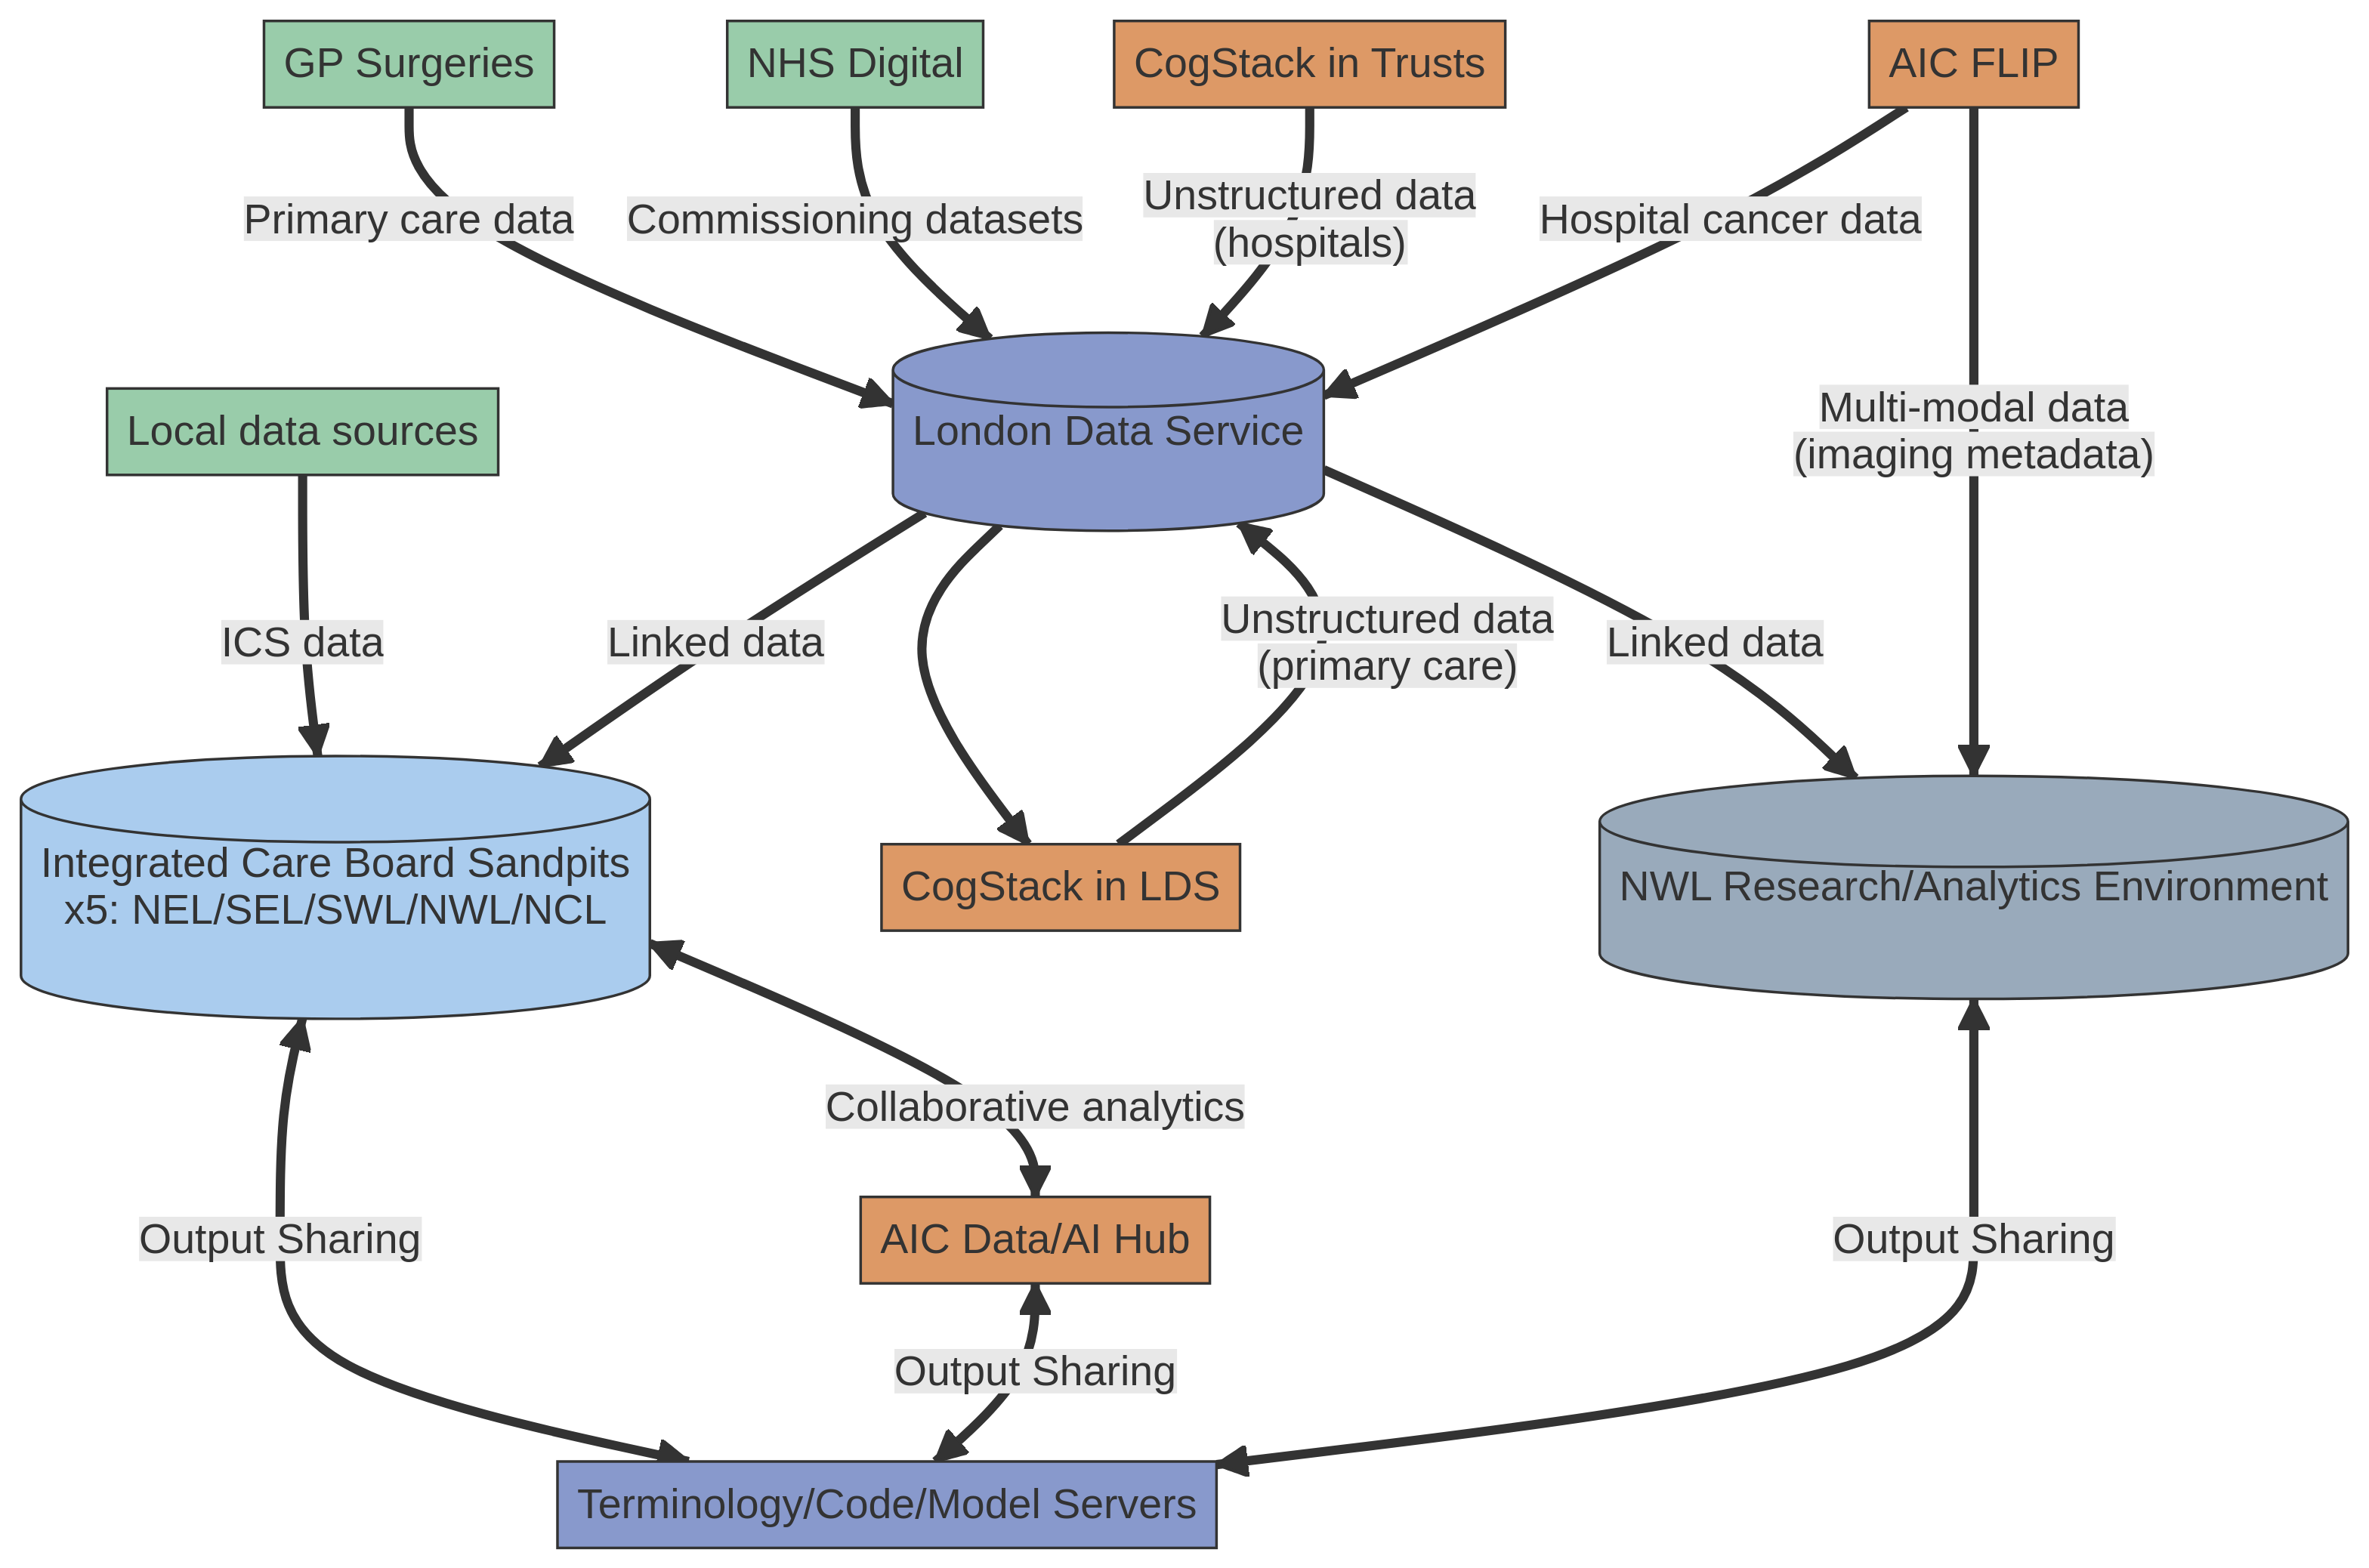
\includegraphics[width=6in,height=3.97in]{index_files/figure-latex/mermaid-figure-4.png}

}

\caption{\label{fig-sde-summary}Summary of SDE components and data
flows. Each London ICB is provisioned with its own data/analytics
environment through the LDS. FLIP = Federated Learning and
Interoperability Platform.}

\end{figure}%

\textsubscript{Source:
\href{https://d3london.github.io/sde_aic_docs/index.qmd.html}{Article
Notebook}}

\subsection{Technology and objectives}\label{technology-and-objectives}

The contribution from the London AIC consists of technology deployment
and supporting expertise, that enable a number of objectives
(Figure~\ref{fig-aic-objectives}) over the two year programme. This
contribution includes the following:

\begin{enumerate}
\def\labelenumi{(\arabic{enumi})}
\item
  \textbf{Federated Learning and Interoperability Platform (FLIP)}:
  Developed and tested over four years, FLIP consists of (a) secure data
  environments within NHS hospital Trusts for multi-modal imaging data,
  imaging metadata, and structured health record data in a common data
  model; and (b) a mechanism to query data and train AI models across
  these secure enclaves without the need to physically transfer data.
  FLIP is presently installed in four major London Trusts. Integrating
  FLIP into the SDE will enable hospital data (such as cancer data) to
  be surfaced into the LDS, and multi-modal capabilities to support
  research in precision healthcare.
\item
  \textbf{CogStack}: As an advanced natural language processing
  platform, CogStack can turn the large quantities of health information
  that are found in narrative text, into structured and analysable data.
  Currently actively used in Trusts to assist with clinical coding from
  notes and clinic letters, CogStack can surface secondary care and
  cancer pathway data, and previously unseen primary care data, into the
  SDE ecosystem.
\item
  \textbf{AIC Data/AI Hub}: The AIC hosts substantial health data and AI
  implementation expertise, that will provide practical support in data
  engineering, clinical informatics, data science, and machine learning
  (ML) development and deployment. Primary aims are to (a) help
  Integrated Care Boards (ICB) migrate data pipelines and analytics onto
  the LDS, (b) produce reproducible analytics pipelines for data science
  and predictive analytics capabilities, (c) work together to make ICBs
  self-sufficient in these capabilities.
\end{enumerate}

\begin{figure}

\centering{

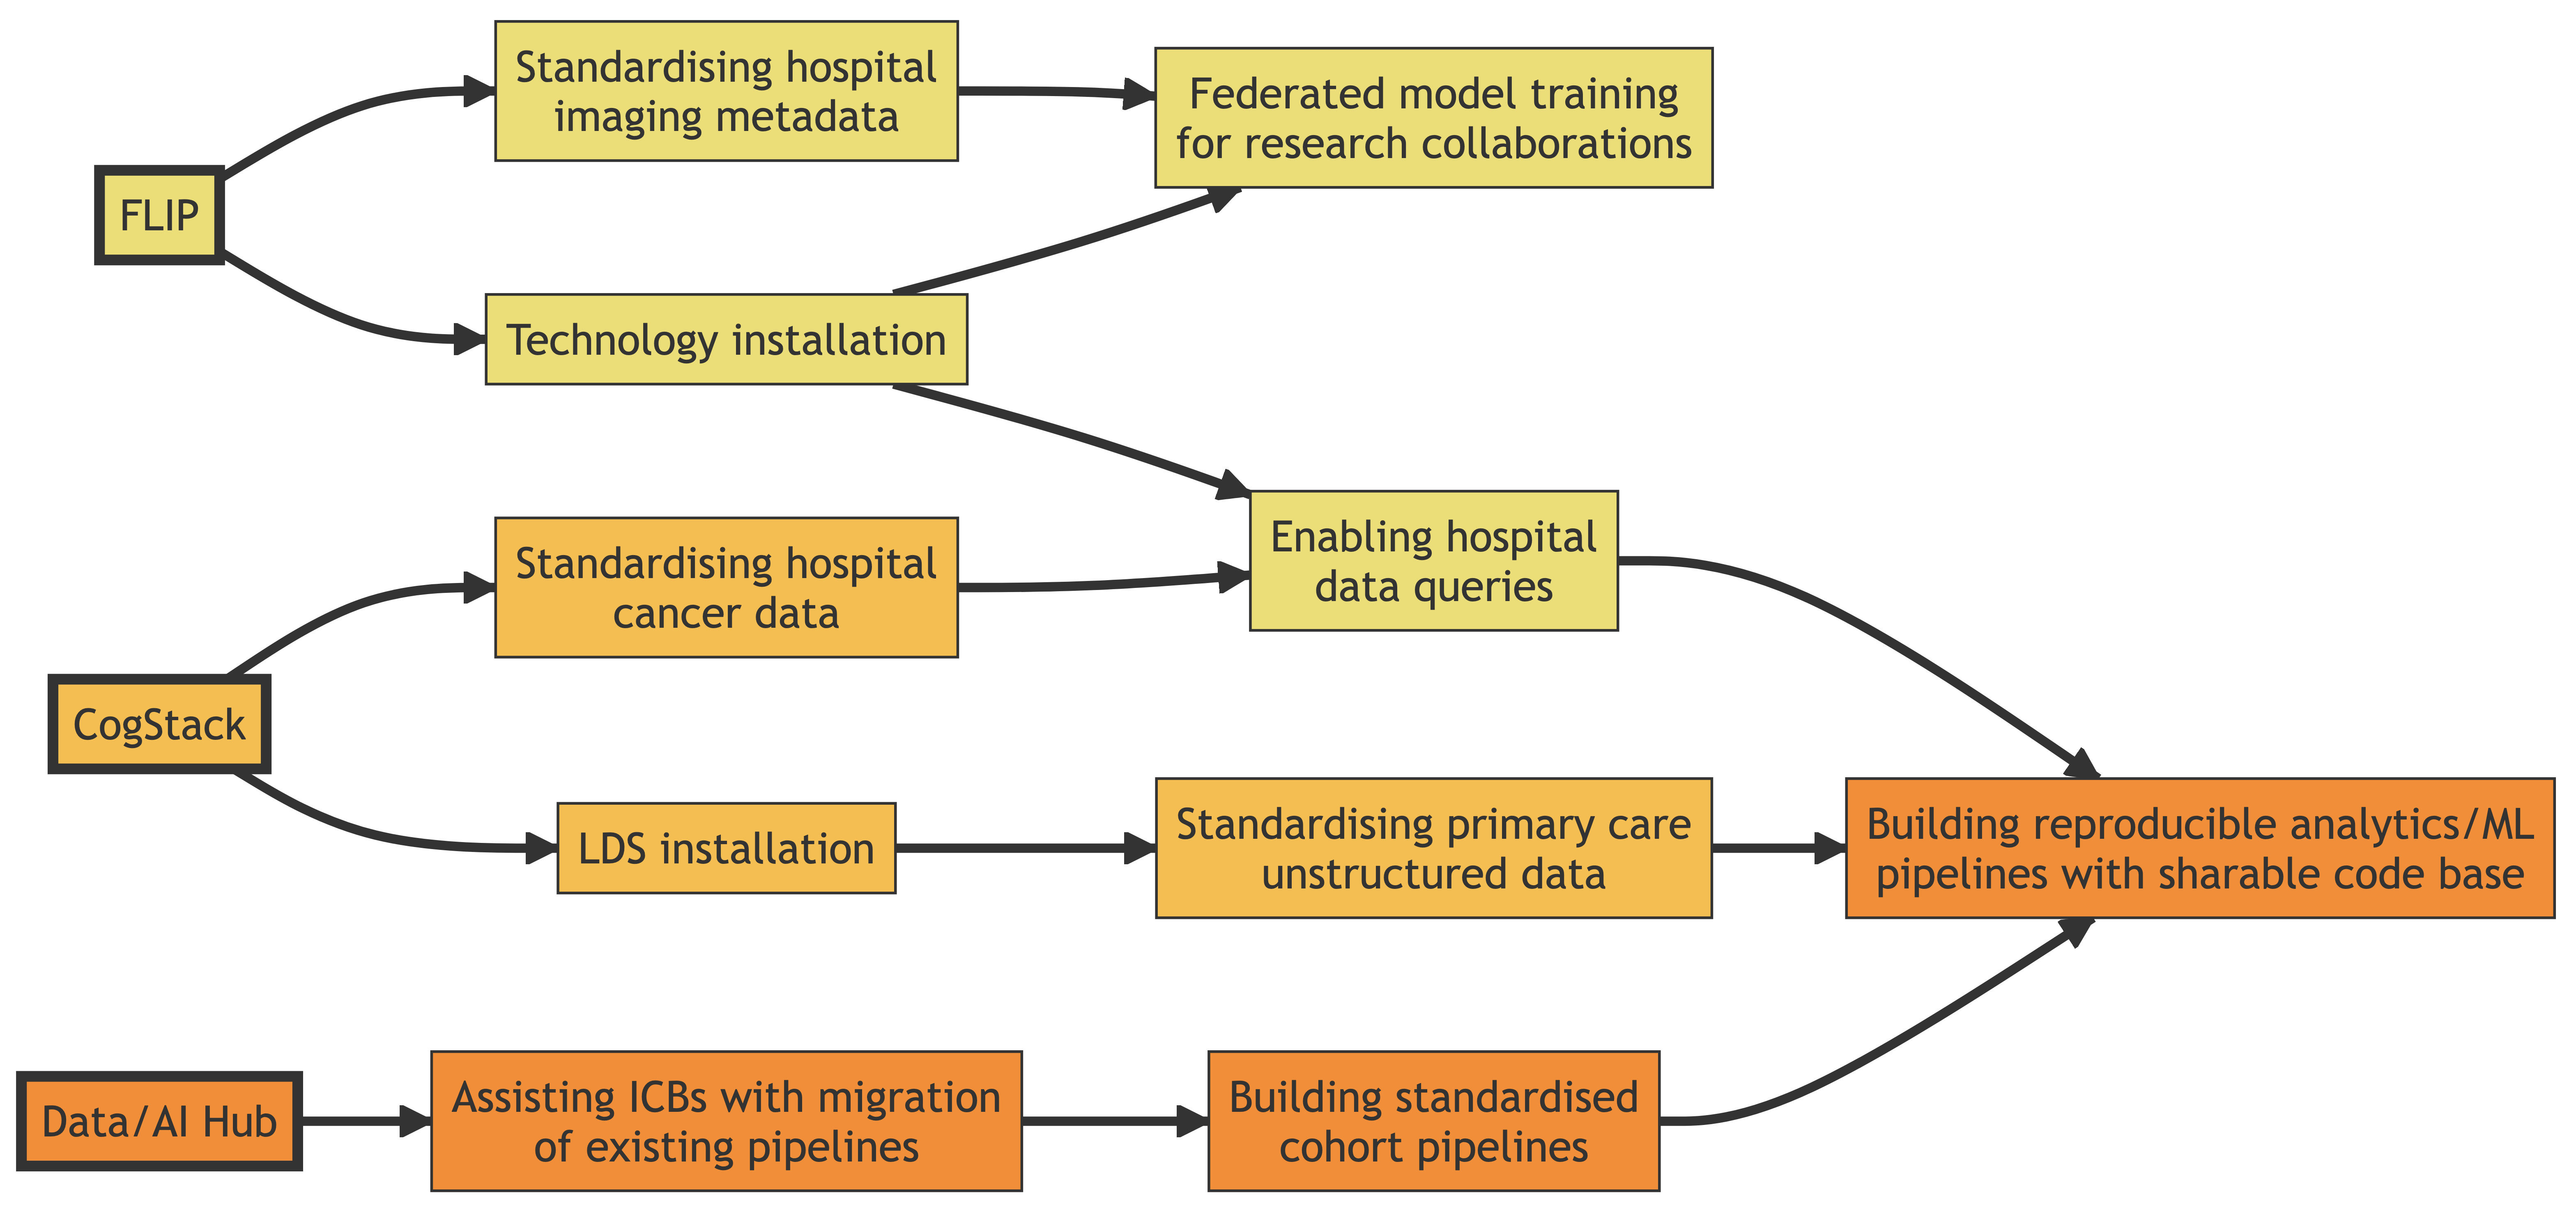
\includegraphics[width=6in,height=2.82in]{index_files/figure-latex/mermaid-figure-6.png}

}

\caption{\label{fig-aic-objectives}Summary of AIC work components and
objectives. FLIP = Federated Learning and Interoperability Platform; ML
= Machine Learning.}

\end{figure}%

\textsubscript{Source:
\href{https://d3london.github.io/sde_aic_docs/index.qmd.html}{Article
Notebook}}

Of relevance to ICBs, resources are available to support migration of
existing analytics into LDS Snowflake `Sandpits', and constructing
standard patient phenotype/cohort using definitions hosted on a London
terminology server. This will support building more complex reproducible
analytics/machine learning pipelines, and delivery of `last mile'
insights to clinicians. As the LDS ICB environments share a common data
model, any pipelines created in collaboration with a single ICB, can be
adapted and used for any other ICB (or deployed across multiple
environments to create pan-London insights). This will also facilitate
shared terminologies, and validating/versioning/serving NHS-owned
machine learning models across regions.

\subsection{Proposed use-cases}\label{proposed-use-cases}

The following use-cases are \emph{examples} of analytics projects that
can be supported within the SDE ecosystem, in collaboration between
ICB/NHS analytics teams and the AIC/SDE team. Use-cases align to the
London Health Data Strategy and long term condition priorities, as well
as national programmes such as CORE20PLUS5, and are proposed here
following early discussions with London ICBs. An overarching objective
for any work is to build a code base that can be shared between ICBs and
improved collaboratively.

\subsubsection{Systematic measurement of group and individual health
inequality}\label{systematic-measurement-of-group-and-individual-health-inequality}

\textbf{AIM:} To systematically surface multiple dimensions of health
inequality across sociodemographic/geospatial groups and individual
patients, and to monitor this data continuously across key long-term
conditions.

\textbf{SUMMARY:} Health inequality refers to measurable differences in
health outcomes and determinants between individuals or groups
(e.g.~morbidity, co-morbidity, disease complications/death, healthcare
access, disease screening, treatment delivery). Where individuals and
groups experience health inequality, the principle of health
\emph{equity} emphases the importance of reducing disparities by
modifying outcome determinants that are unfairly distributed.

Health inequality is traditionally measured and visualised as a
comparison of prevalence/incidence across different population groups.
While helpful for broad insights, this offers limited understanding of
complex individual circumstances. This type of measurement can be
extended to individual patients, by using clinical domain knowledge to
define `indicators' of unequal disease, diagnosis, and treatment
pathways. For example, in an individual with Diabetes Mellitus,
indicators of inequality can include:

Diabetes surfacing at an early age;

Diagnosis in proximity to cardiovascular risk factor co-morbidities;

Diagnosis at a \emph{late} age but with more severe disease, as measured
by HbA1c or presence of end-organ complications;

Reduced health engagement/encounters/treatment compared to what is
expected based on disease severity;

Shorter time to complications and mortality following diagnosis.

The precise contribution of factors to outcomes can be measured and
understood in a multivariate statistical model. Overall, the presence
and magnitude of indicators can be used to visualise, monitor, and
explain different types of inequality, including through comparison of
groups and individuals to `what is expected' in a background population.
The outcome is an increase in actionability, with identification of
modifiable determinants of inequality ( = inequity) for small groups and
individuals.

\textbf{METHODS:} The below shows an example workflow for Diabetes
Mellitus, but can be applied to any long-term condition (not including
cancer).

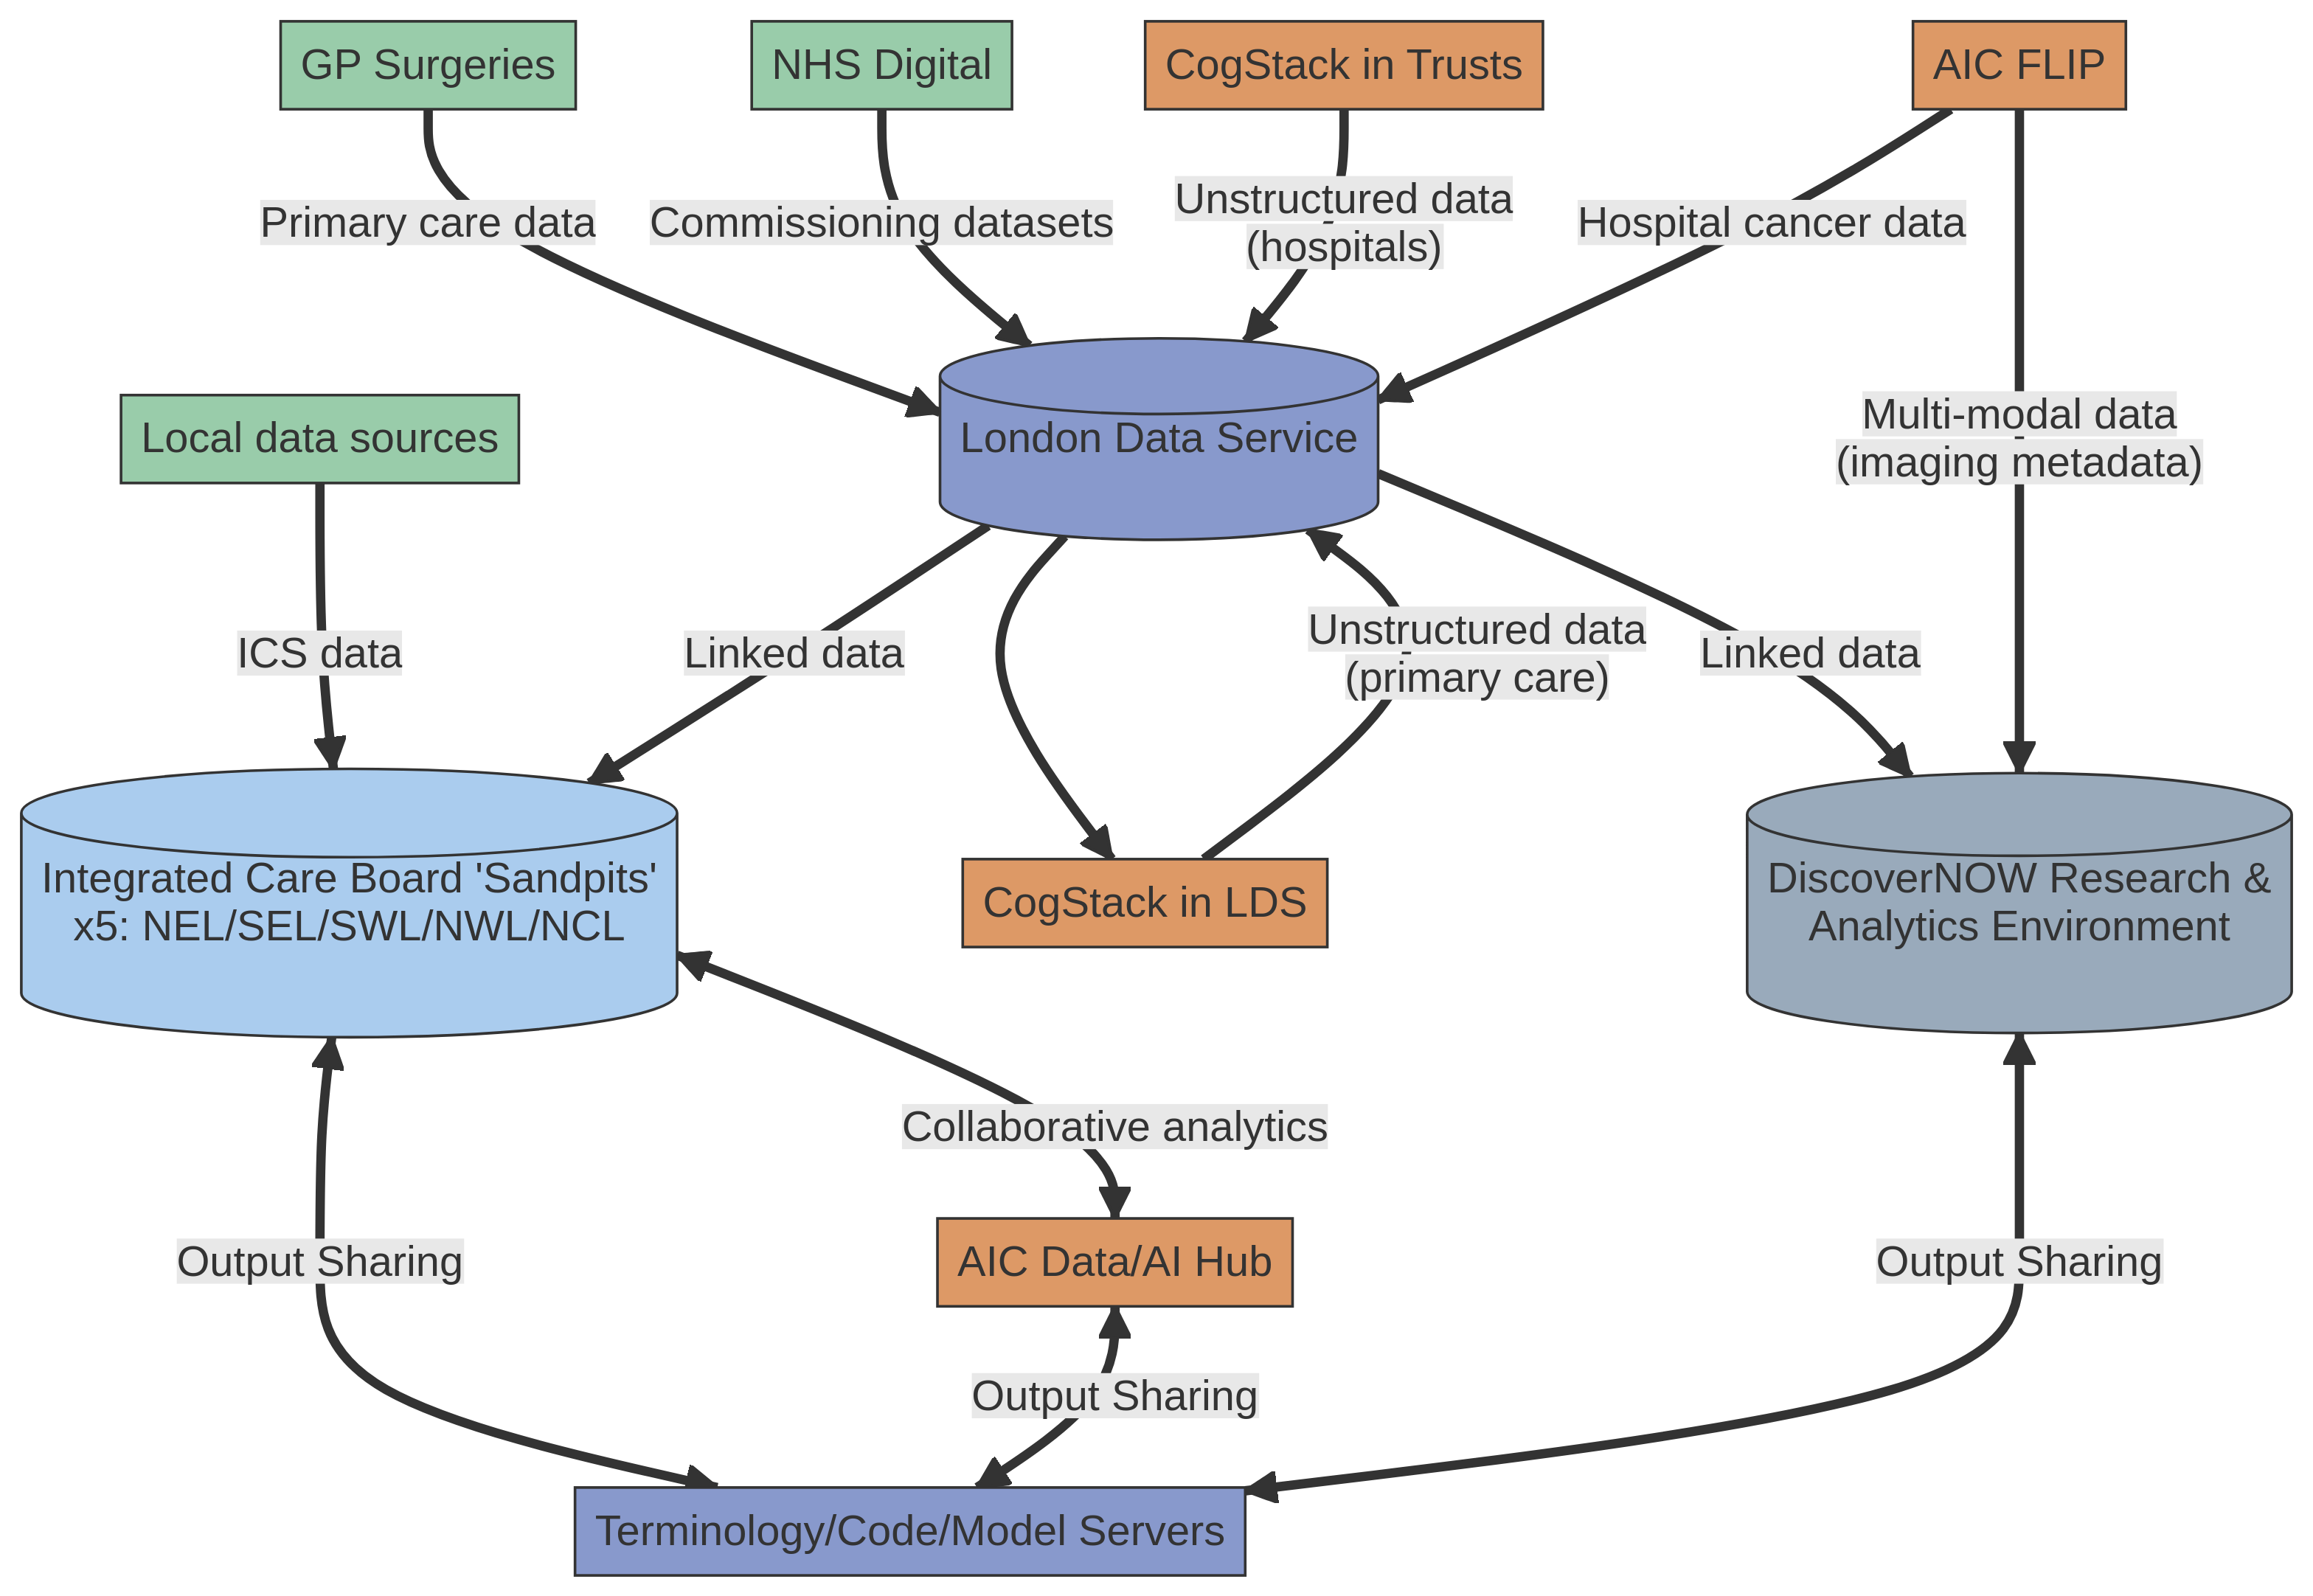
\includegraphics[width=6in,height=1.41in]{index_files/figure-latex/mermaid-figure-5.png}

\textsubscript{Source:
\href{https://d3london.github.io/sde_aic_docs/index.qmd.html}{Article
Notebook}}

\textbf{OUTPUTS:} The primary output of this project would be a
code-base that takes a cohort definition and a list of indicators as an
input, and can be run to produce summary tables and statistics for
groups and individual patients (where required). The code can be adapted
by ICBs and used to support local dashboards. Code can be used for
higher-level interval reporting and monitoring for the London region.

\subsubsection{Cardiovascular disease prevention through decision
intelligence}\label{cardiovascular-disease-prevention-through-decision-intelligence}

\subsubsection{Actionable admission risk
stratification}\label{actionable-admission-risk-stratification}

\subsubsection{Joining up cancer
pathways}\label{joining-up-cancer-pathways}

\subsubsection{}\label{section}



\end{document}
